\chapter{DATA ANALYSIS}\label{ch3}

The first section of this chapter includes an overview of the simulation of the proton-proton collisions and the second section explains the details of the prospects for nonresonant Higgs boson pair production measurements at the HL-LHC in pp collisions with a centre-of-mass energy of $\sqrt{s}=14\;TeV$.

\section{Simulation and Reconstruction of Proton-Proton Collisions}
Monte Carlo event generators are crucial for high energy collision simulations. These software are used by many physicists for many purposes including the anticipation of the design outcomes of colliders. Simulation of a pp collision, interesting for this thesis, starts by describing the hard interactions and moves on to hadronisation and decay. In this section, the working principles of MC simulations for pp collisions are explained.

\subsection{Event generation}

The interactions at the level of partons as well as other subatomic particles, are not deterministic contrary to the classical physics hence the transitions from one quantum state to another is computed as probability. The transition rate $\Gamma_{i\rightarrow f}$ from an initial quantum state $i$ to a final state $f$ is given by the Fermi's Golden Rule as
\be
\Gamma_{i\rightarrow f} = \frac{2\pi}{\hbar}|\mathcal{M}|^2 \rho \; ,
\ee
where $\mathcal{M}$ is the \emph{\bf{Matrix Element}} and is defined as $\langle f|V_i|i\rangle$ for an interaction potential $V_i$. The matrix element describes all the dynamics of the transition and is calculated by evaluating the corresponding Feynman diagrams using the Feynman rules convenient to the interaction of interest. The second ingredient in the recipe is the \emph{phase space} available, also called the \emph{density of final states}, is exclusively kinematic and depends on the masses, energies and momenta of the incident particles. The term represent the phenomenon that the interaction in question is more likely to happen given more space in the final state.

The Golden Rule can be used to cross sections in addition to decay rates. The lowest order term in the perturbation theory calculation for cross section has the highest contribution which is signified as \emph{Leading Order} (LO) and contains only the LO Feynman diagrams. Today, the cross sections are computed using \emph{next-to-leading order} (NLO) calculations in MC event generators which include one-loop diagrams, initial and final state radiations. However, the NLO calculations consume more processor power and time. 

The event generation is the first step of the simulation of the high energy collisions. The Monte Carlo techniques are used to simulate the events which happen in the actual collider experiments. The collisions between the protons at the LHC, takes place in fact between the constituents of the protons, called partons to denote the quark and gluon content. In the pp collisions, not only two partons from different protons collide, which produces an interesting event to study, but also two partons can interact but not hardly. The different types of interactions that may occur in the collisions are shown in \autoref{eventtypes}. The \emph{\bf{hard scattering}} processes occur by the high exchange of momentum between the constituents of two colliding protons. The products of this type of interaction usually have high transverse momenta. The high energetic partons may also emit radiation in the initial and final states, creating parton showers (PS) which is a considerable effect and taken into account in the event generation process.

\begin{figure}[ht]
	\centering
	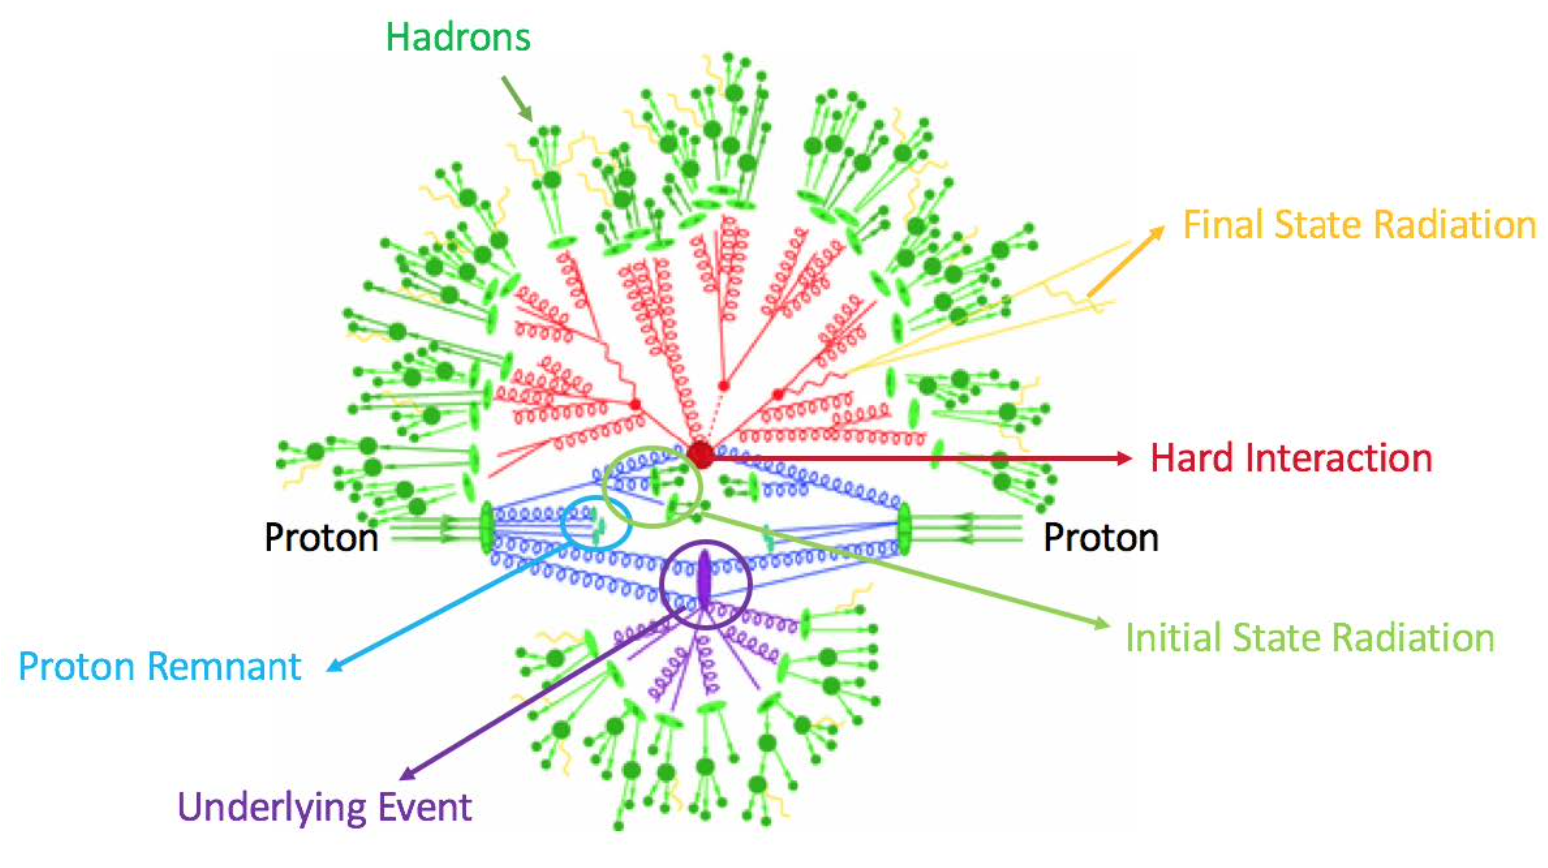
\includegraphics[width=\textwidth]{eventtypes.png}
	\vspace{2mm}
	\caption[Graphical representation of a pp collision event. The proton beams come from the either sides. The red diagram shows the hard interaction and the consequent decay of the products. A secondary interaction before the final state partons hadronise, is shown in purple. The hadronisation is indicated in green.]
	{Graphical representation of a pp collision event. The proton beams come from the either sides. The red diagram shows the hard interaction and the consequent decay of the products. A secondary interaction before the final state partons hadronise, is shown in purple. The hadronisation is indicated in green \cite{Pttgen2016}.}
	\label{eventtypes}
\end{figure}

An \emph{\bf{underlying event}} is a soft interaction that occurs between the residue of the protons which have not taken place in the hard interaction. The partons may also radiate gauge bosons before or after interacting with each other, called initial state radiation and final state radiation, respectively. Additionally, partons can emit radiation via the strong interactions which create jets close to the direction of the initial particles.

At the LHC, bunches including $10^{11}$ protons are collided and pile-up processes, any type of interactions outside the hard scatterings, constitute a significant effect in the event generation. Another aspect of the pp collisions that needs to be considered in MC simulations is the hadronisation process. It is the merger process of quarks and gluons to form colourless, and seen in the final states. The hadronisation process occurs if the partons reach the energy scale of about 1 GeV. The creation of a colourless primary hadrons from partons is described in two different models. The \emph{\bf{cluster model}} describes the forming of the colourless hadrons by the gluons that are split into quark-antiquark pairs which then combines as colourless groups. The states clustered in this manner usually possess a large invariant mass which consequently decay to lower mass states convenient to create hadrons \cite{Webber1984}. In the \emph{\bf{string model}}, the gluons are thought to be split into quark pairs that move away from each other where a string-like configuration is formed between them. As the string is stretched, its potential energy increases lowering the kinetic energy. The string eventually breaks in two creating a quark-antiquark pair. The mechanism is repeated until there is no energy left for another quark pair to be created \cite{Andersson1983}.

Various theoretical, phenomenological and experimental inputs are injected in to MC simulations in order to produce a consistent description of the pp collisions. Different approaches are utilised, for example in order to describe the QCD induced processes which have varying phenomenology with the changing energy scale \cite{skands2012qcd}. The hadronic cross section $\sigma_{pp}$ is calculated using the QCD factorisation theorem, which describing it as a convolution integral of the partonic cross section $\hat\sigma_{ij}$ with the parton distribution functions $f_i(x)$:

\be
\sigma_{pp} = \int_{x_{min}}^1 f_i(x_1)f_j(x_2)\hat\sigma_{ij}(x_1p_1, x_2p_2)dx_1dx_2 \; ,
\ee

where $f_i(x)$ in the probability density that a parton of type $i$ has a fraction x of the hadron's energy.

The overall chain of calculating a process includes;
\begin{itemize}
    \item the PDF, which is basically the phenomenological interpretations calculated with the information coming from the experiments
    \item the hard scattering, calculated in perturbative orders
    \item the parton shower process, the radiations in perturbative QCD
    \item the hadronisation, lays out the forming of colourless hadrons from coloured partons based on phenomenological models
    \item the decay of unstable particles treated using experimental data
\end{itemize}
The first two steps are usually calculated in Matrix Elements generators, while the rest is usually calculated in parton shower software. MC techniques are used in both sides and the transition is made in a manner to avoid double counting of the QCD radiation.

The types on MC generators include general-purpose MC generators which computes the hard processes and the parton shower in seperate structures. \textsc{Pythia8} and \textsc{Sherpa} are most common generators of this group. Other types include generators that compute ME+PS or NLO+PS e.g. \textsc{MadGraph5\_aMC@NLO} which is a unified framework with LO and NLO calculations, and \textsc{Powheg box} which is an ME event generator. The MC event generators used in this thesis is explained later in \autoref{samples_section}.

\subsection{Detector simulation}\label{detector_sim_subsection}

The detector simulation is a crucial step of the simulation of the high energy collisions. It computes the interactions between the particles and the detectors material just as in the actual detector. The final state particles simulated in MC event generators are fed into detector simulations to perform the event reconstruction. There are several detector simulations for high energy collisions. Geometry and Tracking (GEANT4) simulation software \cite{Agostinelli2003}, includes a complete and accurate description of detectors. However, the full simulation of the detector is a long task with high CPU consumption, and in order to cope with the limited computing resources and still allow th use of large samples, the LHC experiments have developed fast simulation software with novel techniques \cite{Sekmen:2242542, Lukas:2012kua} with two to three orders of magnitude faster than GEANT software. In this thesis, all signal and background samples are simulated with the Phase II upgraded CMS detector geometry using \textsc{Delphes} 3 fast simulation \cite{Selvaggi:2014mya}.

\textsc{Delphes 3} aims at simulating multipurpose detector response which includes a track propagation system in the presence of magnetic field, calorimeters and a muon system. It uses the input from the most common event generators and mimics the detector response. In order to achieve this, long-lived particles coming from the hard scattering are propagated through the electromagnetic and hadronic calorimeters withing a uniform magnetic field parallel to the beam line. If the particle is neutral, its trajectory is defined as a straight line from the interaction point to a calorimeter cell. The user may specify the calorimeter segmentation and the magnitude of the magnetic field. After the propagation step, long-lived particles reach the calorimeters, ECAL and HCAL depositing a fixed fraction of their energy. ECAL and HCAL are overlaid and assumed to have same granularity, hence a particle reaches one ECAL and one HCAL cell. These two cells are grouped in a calorimeter tower which is computed as the geometrical centre of the cells. The photons and electrons are defined to deposit all their energy in ECAL with the fraction $f_{ECAL}$, and hadrons in HCAL with $f_{HCAL}$ although in reality hadrons deposit some energy also in ECAL. Muons, neutrinos and neutralinos leave the calorimeters intact and some other particles such as Kaons are treated in a way that they leave their energy in calorimeters instead of decaying. The ECAL and HCAL energy deposits are independently smeared by a log-normal distribution and the energy of each particle is concentrated in one single tower, with the following formula,
\be
E_{tower} = \sum_{particles} ln\mathcal{N} \left( f_{ECAL} \; x \; E,\sigma_{ECAL} \right) + ln\mathcal{N} \left( f_{HCAL} \; x \; E,\sigma_{HCAL} \right) \; ,
\ee
where $ln\mathcal{N}\left(m,s\right)$ is the log-normal distribution with mean $m$ and variance $s$, and the parameters $\sigma_{ECAL}$ and $\sigma_{HCAL}$ are the ECAL and HCAL resolutions given in \autoref{res_eq_ecal}, respectively. The energy of each particle is summed over for a given single tower. High level objects such as jets and missing transverse energy is computed either from the calorimeter deposits or by the particle flow (PF).

\subsection{Particle Flow algorithm}\label{pf_section}

The PF reconstruction, whose philosophy is to use a maximum amount of information obtained from the sub-detectors, is adopted for some experiments including CMS \cite{CMS-PAS-PFT-09-001} and ALEPH \cite{ALEPH:1994ayc}, and is implemented in \textsc{Delphes} with a basic approach based on the tracker and the calorimeter information. In the experiments, the tracker provides a higher resolution than the calorimeters up to some energy scale, therefore \textsc{Delphes} uses the tracker information to calculate the charged particle momenta. The PF algorithm creates two set of 4-vectors; \emph{particle flow tracks} and {particle flow towers. For each calorimeter tower, the algorithm sums the energy deposited in ECAL and HCAL, denoted $E_{ECAL}$ and $E_{HCAL}$ respectively. The total energy deposited by the charged particles for which the tracks have been reconstructed, $E_{ECAL,trk}$ and $E_{HCAL,trk}$ are used in the algorithm to define,

\be
\Delta_{ECAL} = E_{ECAL} - E_{ECAL,trk} \; , \; \Delta_{HCAL} = E_{HCAL} - E_{HCAL,trk} \; ,
\ee
\be
E_{tower} = max(0, \Delta_{ECAL}) + max(0, \Delta_{HCAL})
\label{towerenergy}
\ee

then the algorithm creates a particle flow track for each reconstructed track, and if $E_{tower} > 0$, creates a particle flow tower with $E_{tower}$. In order to illustrate the algorithm with few examples, we can think of a single photon with energy deposited in ECAL with $E_{ECAL}$. A particle flow tower is created for the photon with the deposited energy and no track is created. Another example can be a charged pion with a a track energy $E_{HCAL,trk}$ and with an energy deposit of $E_{HCAL}$. If \autoref{towerenergy} yields zero or a negative value that is $E_{HCAL}\leq E_{HCAL,trk}$, then only a particle flow track with energy $E_{HCAL,trk}$ is created. If $E_{HCAL}\geq E_{HCAL,trk}$, a particle flow track with energy $E_{HCAL,trk}$ along with a particle tower of energy $E_{HCAL}$ is created.

In brief, the particle flow tracks define the charged particles with a good resolution, and particle flow towers define both charged and neutral particles with no relevant tracks characterised by a lower resolution. This approach can be useful for pile-up mitigation, and providing high-resolution input for jet and MET reconstructions. Despite being very plain compared to actual experiments, the PF algorithm is shown to have a good performance at pp collisions \cite{deFavereau2014}. 

\subsection{Reconstruction of physics objects}

\textsc{Delphes} implements the reconstruction and identification of objects based on a set of approximations to reduce the computation time but still keeping a good efficiency.

The \emph{\bf{photon}} reconstruction depends only on the ECAL, and the final energy of the photons is calculated by using the ECAL resolution function presented in \autoref{ecalsubsection}. The photons and electrons that reach ECAL and do not have tracks, are reconstructed as photons in \textsc{Delphes}.

The reconstruction of \emph{\bf{electrons}} is usually performed with the combined information from the tracking system and the ECAL. However, \textsc{Delphes} parametrises the combined reconstruction efficiency as a function of the energy and pseudorapidity instead of dealing with the usual complex reconstruction. The electron reconstruction efficiency drops to zero outside the tracker's geometrical acceptance and below some energy threshold. The energy resolution for the electrons are computed with the combination of tracker resolution at low energies and ECAL resolution at high energies.

The probability for a \emph{\bf{muon}} to be reconstructed in \textsc{Delphes} depends on the user-specified efficiency parametrisation. The probability drops to zero outside the tracker acceptance and below some momenta threshold. The final momentum is computed by a Gaussian smearing of the initial 4 momentum vector of the muon. The resolution is specified by the user as a function of transverse momentum and pseudorapidity.

\emph{\bf{Tau}} leptons decay before being detected, and hereafter, the lepton term is used for electrons and muons. The reconstruction of the hadronically decaying taus will be explained along with jets later.

A photon, electron or muons is said to be isolated if there are small amount of particles around it. The definition of such feature is important since an isolated object is not likely to originate from a jet. Various definitions are available for the isolation of an object. \textsc{Delphes} implements a simple definition that fits well to hadron collisions. An \emph{\bf{isolation}} variable is defined for electrons, muons and photons, as the ratio of the sum of $p_T$ above a threshold in a cone of radius $R$ around a given particle, to the $p_T$ of the particle of interest. The values close to zero signifies that the particle is \emph{isolated}. The user is set free to define parameters of the isolation; $p_T$, $R$ or a minimum isolation, where the default values are $0.1 \; GeV$, 0.5 and 0.1, respectively.

\emph{\bf{Jets}} are produced from three different input collections in \textsc{Delphes}. The \emph{generated jets} are the clusters of generator level long-lived particles after parton- shower and hadronisation. The \emph{calorimeter jets} are produced using calorimeter towers explained in \autoref{detector_sim_subsection}. Finally the \emph{particle flow jets} are the clusters produced fopm the particle flow tracks and towers defined in \autoref{pf_section}. Additionally, the user is set free to specify a minimum jet $p_T$ for the final jet collection, and a jet clustering algorithm with special parameters with The FASTJET package \cite{Cacciari2012} implemented in \textsc{Delphes}, supporting the most common jet clustering algorithms. A default reconstruction step is defined in \textsc{Delphes} that removes the jet from the event if it has been already reconstructed as a lepton or a photon assuring the double counting of objects.

The jets originating from $\tau$ decays or from the the hadronisation of heavy quarks e.g. b or c quarks, should be identified in pp collisions. \textsc{Delphes} tags a jet as b or $\tau$ jet, if the b or $\tau$ is found within some close distance $\Delta R$ of the jet axis, respectively. The user is set free to specify the tagging efficiency which affects the probability of being identified as b or $\tau$. Additionally, a mis-tagging efficiency, that is the probability that a particle other than b or $\tau$ is identified falsely as b or $\tau$.

\textsc{Delphes} is also capable of computing the missing transverse energy $E_T^{miss}$ and scalar transverse energy sum $H_T$.

\subsection{High level corrections and validation}

The reconstructed objects need to be corrected for residual effects before being used in the final analysis. \emph{\bf{Jet energy scale correction}} (JEC) is applied in order to meet the deficit between the average momenta of the reconstructed objects and that of their generator-level equivalent. This deficiency is common for complex objects such as jets, because the total smearing is ambiguous as a result of the loss of generator-level objects such as neutrinos and muons. The JEC is applied therefore applied only on jets, where the user can specify it as a function of $\eta$ and $p_T$ of the reconstructed jet.

The pile-up effects are simulated using a pre-generated QCD, and randomly placed on the beamline with a number obtained from a Poisson distribution. Pile-up has direct effect on the performance of jets, $E_T^{miss}$ and isolation however pile-up mitigation on $E_T^{miss}$ is a demanding task and is not implemented in \textsc{Delphes}. Instead, \emph{\bf{pile-up subtraction}} is applied on jets and the isolation with two methods. \emph{Charged pile-up subtraction} assumes the track reconstruction efficiency does not depend on the vertex position, and if the PF algorithm is used, the PF tracks that originate from pile-up are cleared and do not enter the jet clustering and isolation algorithms. Some other residual effects, e.g. the particles that are in close proximity of the hard interaction vertex, the charged particles that are outside the geometrical acceptance of the tracker, or the neutral particles need to be removed. In order to do this, an average contamination is defined in the \emph{residual pile-up subtraction} which then removed from the jet energies and the isolation variable.

All in all, \textsc{Delphes} has been validated in many use cases, and is a good simulation to be used in pp collisions. \autoref{delphesvalidation} shows a validation plot using photons and electrons vs CMS performance.

\begin{figure}[ht]
	\centering
	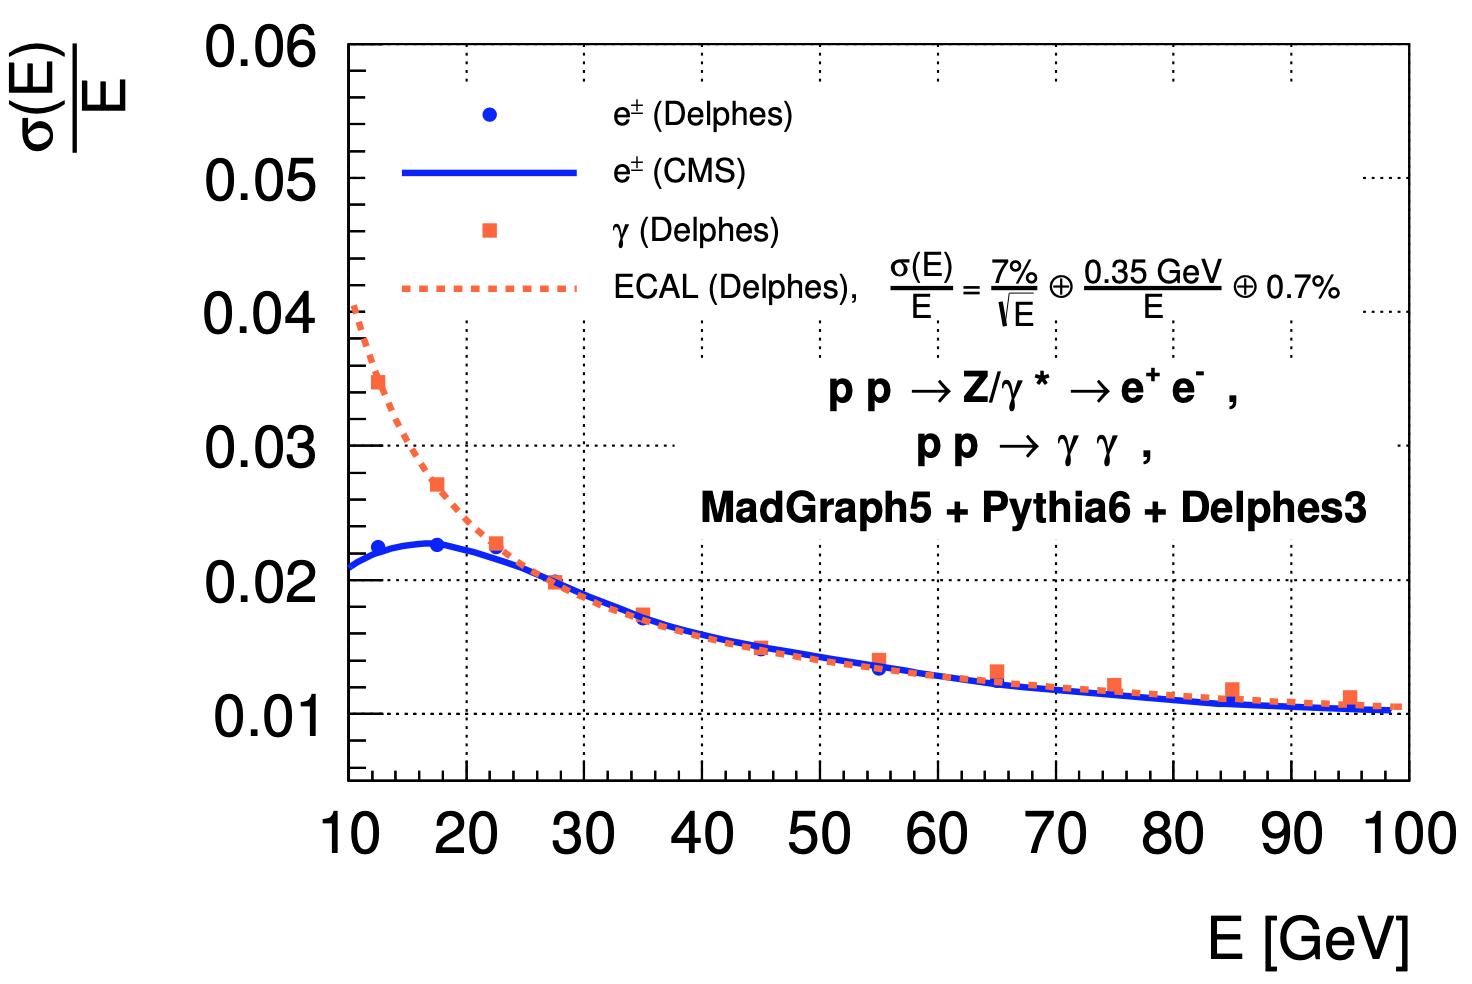
\includegraphics[scale=0.5]{delphesvalidation.png}
	\vspace{2mm}
	\caption[Energy resolution of photons and electrons as a function of energy for a CMS detector configuration.  The energy resolution formula of the CMS ECAL, and the samples used for the study along with their generator are given. The CMS electron distribution is taken from . The electron and photon resolutions are identical at high energies since both objects are dominated by ECAL, however at low energies, the electron resolution differs widely because of the finer tracker resolution.]
	{Energy resolution of photons and electrons as a function of energy for a CMS detector configuration.  The energy resolution formula of the CMS ECAL, and the samples used for the study along with their generator are given. The CMS electron distribution is taken from \cite{CMS:2013hoa}. The electron and photon resolutions are identical at high energies since both objects are dominated by ECAL, however at low energies, the electron resolution differs widely because of the finer tracker resolution \cite{deFavereau2014}.}
	\label{delphesvalidation}
\end{figure}

\section{Higgs Boson Pair Analysis}

This section describes the analysis steps of the prospects for non-resonant Higgs boson pair production measurements at the HL-LHC in pp collisions with a centre-of-mass energy of $\sqrt{s}=14\;TeV$ at the Phase II upgraded CMS detector. In this analysis, a Higgs boson pair search in the \ttgg channel is performed benefiting from the $H\rightarrow \gamma\gamma$ process which provides a clean an distinguishable signature. The final states of Higgs boson pair in \wwgg and \zzgg is included in the study due to overlap, which in turn increases the overall analysis sensitivity. This is the first study providing coupling parameters scan in these channels at the HL-LHC.

The analysis flow is shown in \autoref{analysisflow}.

\begin{figure}[ht]
	\centering
	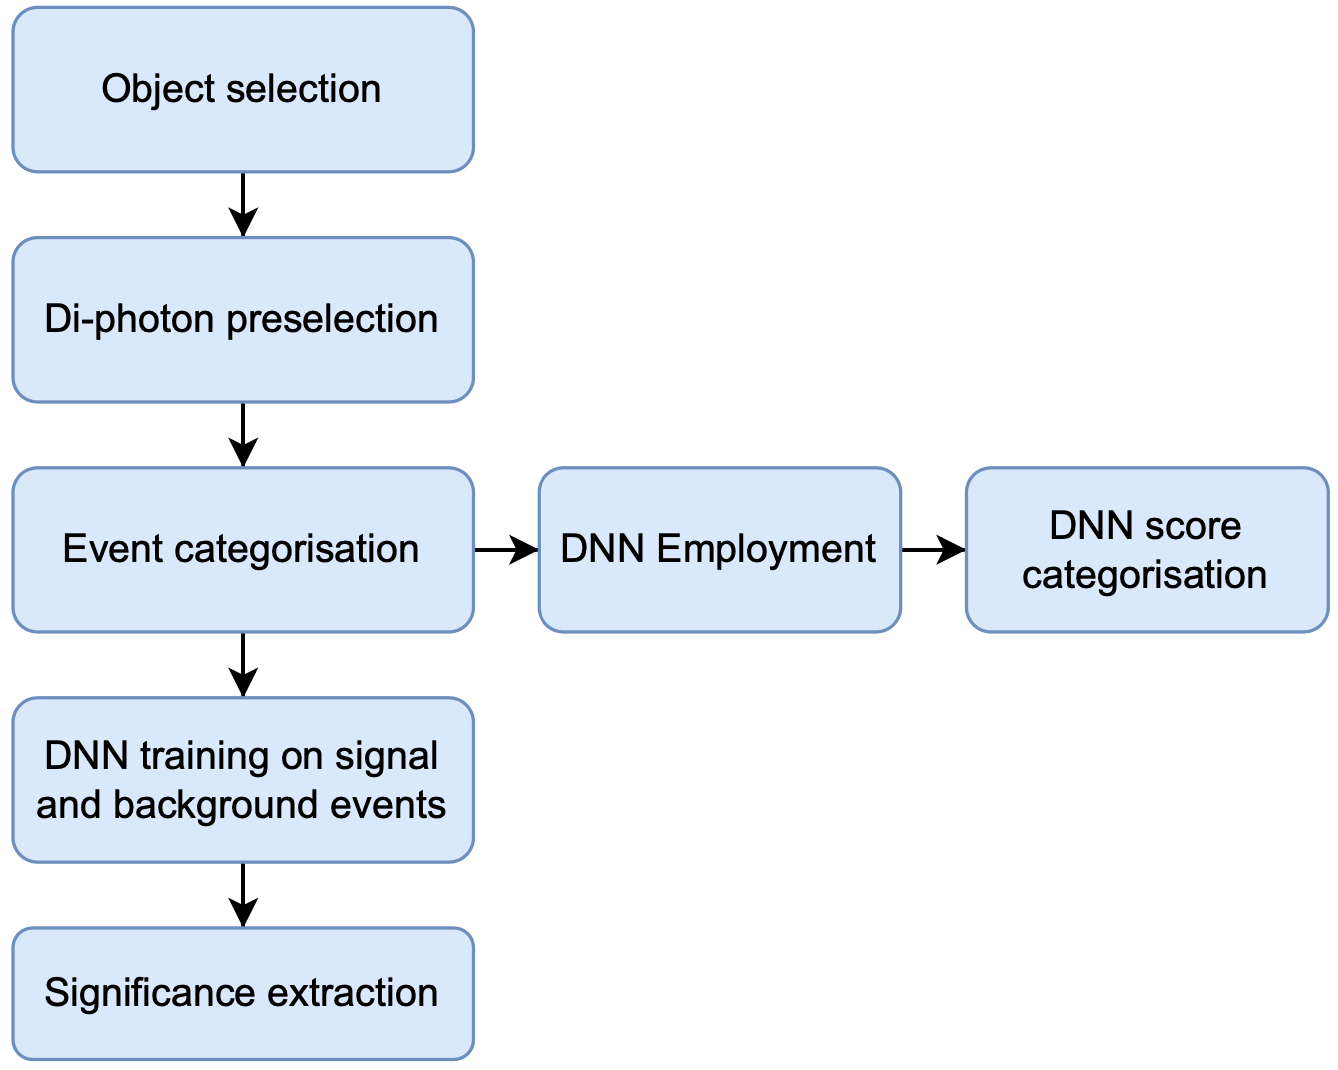
\includegraphics[width=\textwidth]{analysisflow.png}
	\vspace{2mm}
	\caption{Analysis flow chart.}
	\label{analysisflow}
\end{figure}

\subsection{Signal and background samples}\label{samples_section}

In this thesis, signal ($gg \rightarrow HH$) samples are generated using \textsc{Powheg v2} \cite{Nason2004, Frixione2007, Alioli2010, Heinrich2019} at next-to-leading order (NLO) in QCD including the full top mass dependence with SM parameters, and subsequent decays of the Higgs boson pairs into $\tau\tau$, $WW$ and $ZZ$ each with a photon pair is implemented using \textsc{Pythia 8.212} \cite{Sjstrand2015}. The signal samples for three separate final states of \wwgg channel are produced while a single sample including all possible decays of taus are used.

The analysis is overwhelmed by non-resonant backgrounds with continuum \mgg spectra and by single Higgs boson productions. The sample generation for single Higgs productions is performed via \textsc{MadGraph5\_aMC@NLO} \cite{Alwall2014, Artoisenet2013} with the FxFx merging scheme \cite{Frederix2012} for the gluon fusion (ggFH), vector boson fusion (VBFH), associated production with a vector boson (VH) and associated production with a top quark pair (ttH), while the top quark associated production  with a Higgs boson (tHq) was performed using \textsc{MadGraph} version-2.7 at LO.

Several SM processes contribute to the continuum background. A large portion of the dominant backgrounds across all final states comes from the $\gamma\gamma+$jets processes that are modelled with \textsc{Sherpa} v.2.2.1 generator \cite{10.21468/SciPostPhys.7.3.034} while QCD-induced processes, $\gamma+$jets and WW processes are modelled with \textsc{Pythia} 8 generator. W production in association with photons and jets, and Drell-Yan processes are modelled with \textsc{MadGraph5} version-2.7 at LO, $t\bar t$ with \textsc{Powheg} v2, and $t\bar tW$, $t\bar t\gamma$, $t\bar t\gamma\gamma$, $Z\gamma$ processes with \textsc{MadGraph5\_aMC@NLO}. A complete list of samples used in the analysis is shown in \autoref{MCSamples}.

\begin{table}[h!]
    \resizebox{\textwidth}{!}{
      \begin{tabular}{lcc}
        \hline \hline
        Dataset & Nevents & X-section $\times$ BR (fb)\\
        \hline
        \multicolumn{3}{c}{Signal} \\
        \hline
      $GluGluToHHTo2G2Tau\_node\_cHHH1\_TuneCP5\_14TeV$-$powheg$-$pythia8\_200PU$ & 1999866 & 0.00104441\\
      $GluGluToHHTo2G2Qlnu\_node\_cHHH1\_TuneCP5\_14TeV$-$powheg$-$pythia8\_200PU$ & 1898894 & 0.0156981\\
      $GluGluToHHTo2G2l2nu\_node\_cHHH1\_TuneCP5\_14TeV$-$powheg$-$pythia8\_200PU$ & 1885835 & 0.0037234\\
      \multicolumn{3}{c}{Resonant Background} \\
      \hline

      $VHToGG\_M125\_TuneCP5\_14TeV$-$amcatnloFXFX$-$madspin$-$pythia8\_200PU$ & 1830426 & 5.44326\\
      $ttHJetToGG\_M125\_TuneCP5\_14TeV$-$amcatnloFXFX$-$madspin$-$pythia8\_200PU$ & 5971707 & 1.393764\\
      $GluGluHToGG\_M125\_TuneCP5\_14TeV$-$amcatnloFXFX$-$pythia8\_200PU$ & 444658 & 114.798\\
      $VBFHToGG\_M125\_TuneCP5\_14TeV$-$amcatnlo$-$pythia8\_200PU$ & 1712900 & 9.51216\\
      $THQ\_ctcvcp\_HToGG\_M125\_TuneCUETP8M1\_14TeV$-$madgraph$-$pythia8\_200PU$ & 789129.0 & 0.205428 \\ 
      
      \multicolumn{3}{c}{Continuum Background} \\
      \hline
      $DiPhotonJetsBox\_MGG$-$40to80\_14TeV$-$Sherpa\_200PU$ & 20677034.0 & 332804\\ 
      $DiPhotonJetsBox\_MGG$-$80toInf\_14TeV$-$Sherpa\_200PU$ & 19933297 & 98670\\
      $GJet\_Pt$-$20toInf\_DoubleEMEnriched\_MGG$-$40to80\_TuneCUEP8M2T4\_14TeV\_pythia8\_200PU$ & 19985496 & 3901000\\
      $GJet\_Pt$-$40toInf\_DoubleEMEnriched\_MGG$-$80toInf\_TuneCUEP8M2T4\_14TeV\_Pythia8\_200PU$ & 20033932 & 998100\\
      $GJet\_Pt$-$20to40\_DoubleEMEnriched\_MGG$-$80toInf\_TuneCP5\_14TeV$-$pythia8\_200PU$ & 14313734 & 260850\\
      $QCD\_Pt$-$30toInf\_DoubleEMEnriched\_MGG$-$40to80\_TuneCUEP8M2T4\_14TeV\_Pythia8\_200PU$ & 19581853 & 295700000\\
      $QCD\_Pt$-$40toInf\_DoubleEMEnriched\_MGG$-$80toInf\_TuneCUEP8M2T4\_14TeV\_Pythia8\_200PU$ & 7141716 & 141200000\\
      $QCD\_Pt$-$30to40\_DoubleEMEnriched\_MGG$-$80toInf\_TuneCUEP8M2T4\_14TeV\_Pythia8\_200PU$ & 30793791 & 16510000\\
      
      $TT\_TuneCUETP8M2T4\_14TeV$-$powheg$-$pythia8\_200PU$ & 49398942 & 864400\\
      $TTWJetsToLNu\_TuneCUETP8M1\_14TeV$-$amcatnloFXFX$-$madspin$-$pythia8\_200PU$ & 5040836.0 & 225.3 \\ 
      $TTGamma\_Dilept\_TuneCUETP8M2T4\_14TeV$-$madgraph$-$pythia8\_200PU$ & 2999843 & 623.1\\
      $TTGamma\_Hadronic\_TuneCUETP8M2T4\_14TeV$-$madgraph$-$pythia8\_200PU$ & 2999836 & 799\\
      $TTGamma\_SingleLeptFromT\_TuneCUETP8M2T4\_14TeV$-$madgraph$-$pythia8\_200PU$ & 2939839 & 770.9\\
      $TTGamma\_SingleLeptFromTbar\_TuneCUETP8M2T4\_14TeV$-$madgraph$-$pythia8\_200PU$ & 2939844 & 769\\
      $TTGG\_0Jets\_TuneCUETP8M1\_14TeV\_amcatnlo\_madspin\_pythia8\_200PU$ & 1101895 & 18.64\\
      
      $DYJets\_incl\_MLL$-$50\_TuneCUETP8M1\_14TeV$-$madgraphMLM$-$pythia8\_200PU$ & 76952612.0 & 5711000 \\ 
      $W1JetsToLNu\_TuneCUETP8M1\_14TeV$-$madgraphMLM$-$pythia8\_200PU$ & 77486992.0 & 10370000  \\ 
      $W2JetsToLNu\_TuneCUETP8M1\_14TeV$-$madgraphMLM$-$pythia8\_200PU$ & 43222285.0 & 2965000  \\ 
      $W3JetsToLNu\_TuneCUETP8M1\_14TeV$-$madgraphMLM$-$pythia8\_200PU$ & 5674591.0 & 1268000 \\ 
      $WGToLNuG\_PtG$-$40\_TuneCUETP8M1\_14TeV$-$madgraphMLM$-$pythia8\_200PU$ & 11776400 & 18790\\
      $ZGTo2LG\_TuneCUETP8M1\_14TeV$-$amcatnloFXFX$-$pythia8\_200PU$ & 30301987 & 145200\\
      $WGGJets\_TuneCP5\_14TeV\_madgraphMLM\_pythia8\_200PU$ & 1981569.0 & 1884 \\ 
      $WGJJToLNu\_EWK\_QCD\_TuneCP5\_14TeV$-$madgraph$-$pythia8\_200PU$ & 1801596.0 & 6032 \\ 
      $WW\_TuneCUETP8M1\_14TeV$-$pythia8\_200PU$ & 99484471.0 & 70440\\ 
      \hline
      \end{tabular}
       }
        \caption{MC samples used in the analysis.}
        \label{MCSamples}
    \end{table}

In this thesis, all signal and background samples are simulated with the Phase II upgraded CMS detector geometry using \textsc{Delphes} 3 fast simulation \cite{Selvaggi:2014mya} with an average pile-up of 200 interactions at $\sqrt{s}=14$ TeV. An Ntupliser is used to produce flat Ntuples using the outputs from \textsc{Delphes}, whose form is shown in \autoref{flattree}.

\begin{figure}[ht]
	\centering
	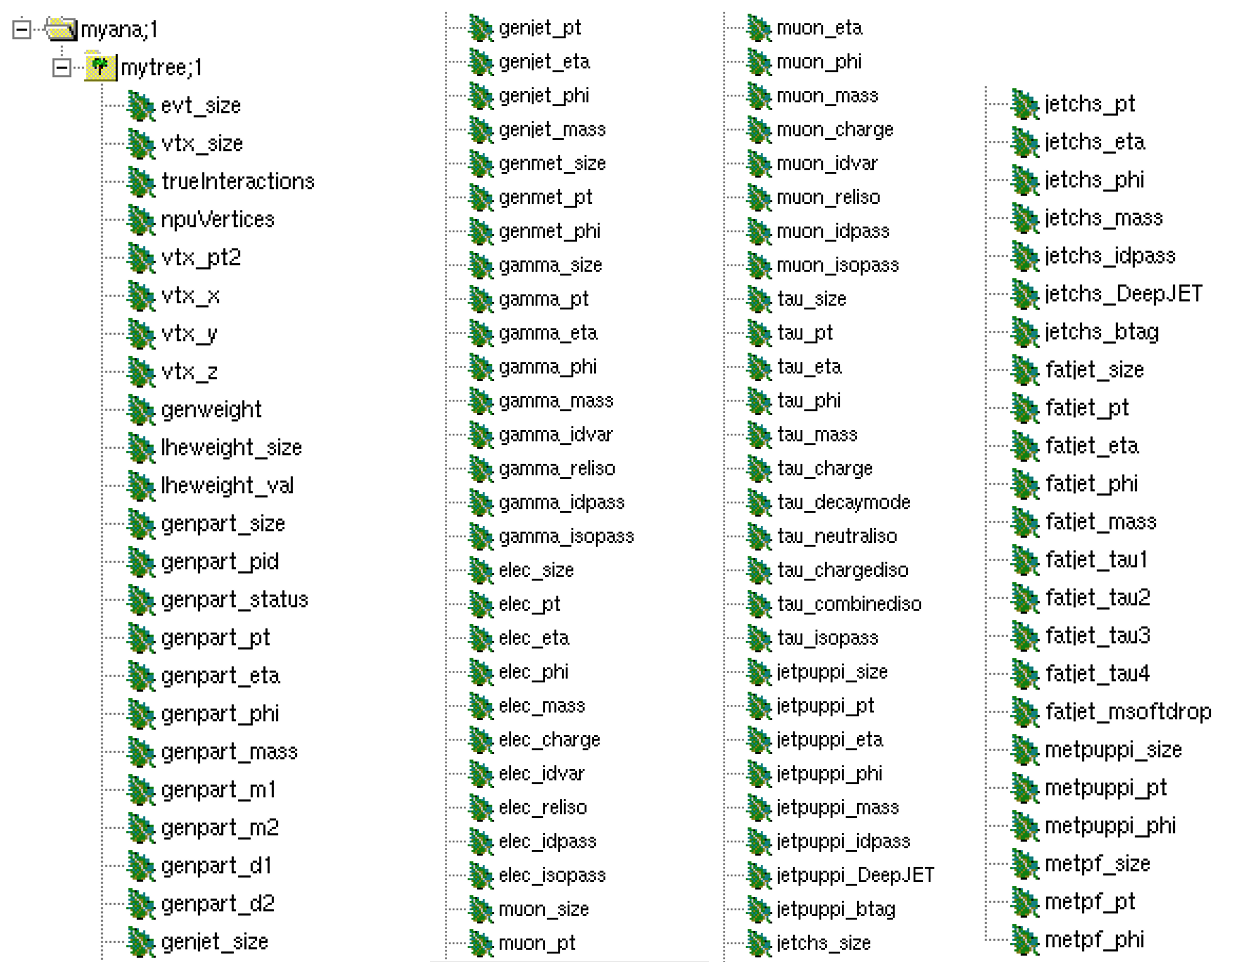
\includegraphics[width=\textwidth]{flattree.png}
	\vspace{2mm}
	\caption[The flat tree format of the \textsc{Delphes} simulated samples. The reconstructed objects include photons, electrons, muons, taus, jets and $E_T^{miss}$. Each object has the multiplicity, mass, $p_T$, $\eta$, $\phi$ values except $E_T^{miss}$ which do not have mass and $\eta$ values. Identification and isolation variables are available for most of the objects and b-originated jets information is available for jets. There is also the possibility to work on the generator level with generated particles (genpart), jets (genjet) and $E_T^{miss}$ (genmet) collections. Genparts collection possess mother (m1, m2) and daughter (d1, d2) particles information along with particle status codes (PID). Jets and $E_T^{miss}$ have different versions produced used different algorithm, i.e. pile-up per particle identification (PUPPI), charged hadrons subtracted (CHS) or particle flow (PF). Additionally, number of events, vertex information, generator level weight are among the accessible information.]{The flat tree format of the \textsc{Delphes} simulated samples. The reconstructed objects include photons, electrons, muons, taus, jets and $E_T^{miss}$. Each object has the multiplicity, mass, $p_T$, $\eta$, $\phi$ values except $E_T^{miss}$ which do not have mass and $\eta$ values. Identification and isolation variables are available for most of the objects and b-originated jets information is available for jets. There is also the possibility to work on the generator level with generated particles (genpart), jets (genjet) and $E_T^{miss}$ (genmet) collections. Genparts collection possess mother (m1, m2) and daughter (d1, d2) particles information along with particle status codes (PID). Jets and $E_T^{miss}$ have different versions produced with different algorithm, i.e. pile-up per particle identification (PUPPI) \cite{puppi}, charged hadrons subtracted (CHS)\cite{jetchs} or particle flow (PF). Additionally, number of events, vertex information, generator level weight are among the accessible information.}
	\label{flattree}
\end{figure}

For the Phase II upgraded CMS detector configuration in \textsc{Delphes} input card \cite{delphescard}, the isolation (ISO) and identification (ID) variables for photons and electrons are defined in different bit-wise working points (WP); loose, medium and tight (LMT) based on the MVA trained ID and ISO variables in full simulation of CMS (FullSim). Similar ID and ISO variables are defined for muons and taus, and a \emph{btag} value in bit-wise LMT WPs is also defined for jets.

\subsection{Object selection}

Photons used in this analysis are required to have a $p_T$ above 25 GeV and be in the geometrical acceptance that is $|\eta| < 3$. The photon with the highest \pt in the events, namely the leading photon is required to have a \pt of at least 35 GeV. The relative isolation ISO, defined as the sum of transverse momenta of all the particles within a particular size of cone divided by the \pt of the particle of interest, is required to be less than 0.3 for photon candidates. A bit-wise criteria, 1, 3, 7 for loose, medium, tight, respectively, is applied in order to select the loose-ID photons. The photons that pass all these selections are called \emph{good photons} hereafter.

Electrons are required to have transverse momenta above 10 GeV within $|\eta|<3$ region. The electrons and good photons are isolated from each other with an angular separation of at least 0.4. The muons that have at least 10 GeV \pt and in $|\eta|<2.8$ have been selected and they are isolated from the good electrons and good muons with an angular separation greater than 0.2. Tau leptons with $p_T > 20$ GeV are used in $|\eta|<3$ and are cleaned with respect to good photons/electrons/muons. PUPPI-jets that have $p_T > 30$ GeV with $|\eta|<5$ are used with an angular separation of 0.4 with respect to good photons/electrons/muons/taus. A list of all selections is shown in \autoref{seltable}.

\begin{table*}[ht]
	{\setlength{\tabcolsep}{14pt}
		\caption{Object selections.}
		\begin{center}
			\vspace{-6mm}
			\begin{tabular}{lcccc}
				\hline \\[-2.45ex] \hline \\[-2.1ex]
				Object & \pt $\left[GeV\right]$ & $|\eta|$ & ($\Delta R$) w.r.t. & Working Point \\
				\hline \\[-1.8ex]
                Photon ($\gamma$) & 25 & 3 & - & loose ISO+ID \\
                Electron ($e$) & 10 & 3 & $\gamma$ (0.4) & loose ISO+ID \\
                Muon ($\mu$) & 10 & 2.8 & $e$, $\gamma$ (0.2) & tight ISO+ID \\
                Tau ($\tau$) & 20 & 3 & $e$,$\gamma$,$\mu$ (0.2) & tight ISO \\
                Jet & 30 & 5 & $e$,$\gamma$,$\mu$,$\tau$ (0.4) & tight ID, medium btag \\
				\hline
			\end{tabular}
			\vspace{-6mm}
		\end{center}
		\label{seltable}}
\end{table*}

\subsection{Event selection and categorisation}

All events in the analysis are required to have the invariant mass of two good photons within $100<\mgg<180$ GeV as a preselection for all final states. The analysis is performed in several non-overlaping (orthogonal) final states targeting the decays of the W bosons referred to as \emph{semi-leptonic} and \emph{fully-leptonic} final states for \wwgg, and 1$\tau$ and 2$\tau$ final states for \ttgg. Full hadronic final state of \wwgg is not included in this thesis due to modelling difficulties in QCD induced background samples.

In the \emph{\bf{semi-leptonic final state}}, the events that contain at least one good photon pair (the preselection) and exactly one good electron or good muon are selected. This final state is expected to be the most sensitive of the two \wwgg final states due to the mix of a high energy lepton from the $W\rightarrow l\nu$ decay with the relatively large branching fraction of the $W\rightarrow qq$ leg of the decay.

In order to separate the Higgs pair signal from the resonant background (Single Higgs boson production for our case) and the continuum background, two multiclass \emph{\bf{Deep Neural Networks}} (DNN) are employed. Due to the imbalance between the two classes caused by the dataset, event weights are first scaled to the expected cross sections, then reweighted so that the learning weight in the classes became similar. This assured the nueral networks to focus on categorising the two classes with equal improtance. In order to avoid training bias in the DNN, the data is divided into almost two equal parts based on the fifth decimal place of the leading good photon's $\phi$ value. The output sets are labelled as \emph{even} and \emph{odd} according to the chosen decimal, and the DNN performed with the even set is applied on the odd set.

The framework choise for the DNN is the \textsc{TensorFlow} \cite{tensorflow}, which is an open source software library for machine learning that can be used in a wide variety of programming languages; Python, Javascript, C++, and Java. \textsc{Keras} \cite{keras} is the interface chosen to be used with \textsc{TensorFlow}. The reason to choose these software is that they are compatible with \textsc{Python} programming language. Additionally, both systems can run on both CPU and GPU which makes them very fast, and there is a large community working on them which makes it easy to find solutions to the problems encountered in the DNN training. Another reason to use these software is the compatibility between them and the analysis framework called \textsc{Bamboo} \cite{bamboo}. It is a high-level HEP analysis library built on top of \textsc{Root}'s \emph{RDataFrame} class. \emph{RDataFrame} offers a modern, high-level interface for analysis of data stored in TTree other data formats, in Python or C++. TTree is the data format of our samples, and since \textsc{Bamboo} is built using \textsc{Python} language, the whole analysis and DNN frameworks work in good harmony. 

The feature variables used as input ot train the DNN include the kinematic variables such as \pt, $\eta$, $\phi$ and energy values of objects along with the reweighted variables. The full list of input features is given in \autoref{dnninputs}. The resulting DNN score distribution is shown in \autoref{..}.

\begin{table}[h!]
    \caption{Input features used to train semi-leptonic final state DNN.}
    \resizebox{\textwidth}{!}{
    \begin{tabular}{ l | l }
    \hline
    Feature & Description \\
    \hline
    Leading Photon p$_T$ / \mgg& \pt of the leading good photon scaled to diphoton mass. \\
    Leading Photon $\eta$ & Pseudorapidity of the leading good photon \\
    Leading Photon $\phi$ & Direction in the transverse plane of the leading good photon\\
    Leading Photon E / \mgg& Energy of the leading good photon scaled to diphoton mass. \\
    Sub-leading Photon p$_T$  / \mgg& \pt of the sub-leading good photon scaled to diphoton mass.\\
    Sub-leading Photon $\eta$ & Pseudorapidity of the sub-leading good photon\\
    Sub-leading Photon $\phi$ & Direction in the transverse plane of the sub-leading good photon\\
    Sub-leading Photon E / \mgg & Energy of the sub-leading good photon scaled to diphoton mass. \\
    Jet Multiplicity & Number of selected jets in the event (flavour inclusive) \\
    Leading Jet p$_T$ & \pt of the leading good jet \\
    Leading Jet $\eta$ & Pseudorapidity of the leading good jet \\
    Leading Jet $\phi$ & Direction in the transverse plane of the leading good jet \\
    Leading Jet E & Energy of the leading good jet \\
    Leading Jet btag & b-tag discriminator of the leading good jet \\
    Sub-leading Jet p$_T$ & \pt of the sub-leading good jet \\
    Sub-leading Jet $\eta$ & Pseudorapidity of the sub-leading good jet \\
    Sub-leading Jet $\phi$ & Direction in the transverse plane of the sub-leading good jet \\
    Sub-leading Jet E & Energy of the sub-leading good jet \\
    Sub-leading Jet btag & b-tag discriminator score of the sub-leading good jet \\
    Electron p$_{T}$ & \pt of the selected electron \\ 
    Electron $\eta$ & Pseudorapidity of the selected electron \\ 
    Electron $\phi$ & Direction in the transverse plane of the selected electron \\ 
    Electron E & Energy of the selected electron  \\ 
    Muon p$_{T}$ & \pt of the selected muon \\ 
    Muon $\eta$ & Pseudorapidity of the selected muon \\ 
    Muon $\phi$ & Direction in the transverse plane of the selected muon \\ 
    Muon E & Energy of the selected muon \\ 
    MET & Missing transverse energy in the event \\ 
    $m_{j_{0},j_{1}}$ & The invariant mass of the leading and sub-leading jets \\ 
    \hline
    \end{tabular}
    }
    \label{dnninputs}
\end{table}



\subsection{Systematic uncertainties}

\section{Results}